\documentclass[10pt,fleqn,a4paper]{article}
\usepackage{encit2010}
\usepackage{amsmath}
\usepackage{amsthm}

\newcommand{\bv}[1]{\mathbf{#1}}
\newcommand{\xp}{x^{\mathbf{\prime}}}
\newtheorem{theorem}{Theorem}

% LEGEND FOR THE GEOMETRIES
% Action = Head 1
% Scania = Head 2
% Sygma = Head 3
% Ducato = Head 4


\begin{document}
\hspace{-8.5mm}
\begin{tabular}{||p{\textwidth}}
\begin{center}
\vspace{-4mm}
\title{ANALYSIS OF STEREOSCOPIC PIV MEASUREMENTS OF IN-CYLINDER FLOWS USING PROPER ORTHOGONAL DECOMPOSITION}
\end{center}
\authors{Rodrigo Piccinini, rodrigo.piccinini@sygmamotors.com.br} \\
\authors{Carla Fernandes, carla.fernandes@sygmamotors.com.br} \\
\authors{Marcelo Andreotti, marcelo.andreotti@sygmamotors.com.br} \\
\institution{Sygma Motors, Av. Cassiano Ricardo, 1306, sala 2, Jardim Alvorada, CEP 12240 - 540, S\~{a}o Jos\'{e} dos Campos - SP - Brasil} \\
\\
\abstract{\textbf{Abstract} 

% SHORT ABSTRACT

%In the present work, the Proper Orthogonal Decomposition (POD) was applied in the
% identification of flow coherent structures. The experiment consisted of 
% mounting on an Plexiglas cylinder the intake ports of an internal 
% combustion engine and establishing a steady flow through this system.
%Velocity fields at different cylinder cross sections and for several 
%instants of time were measured by Particle Image Velocimetry (PIV).
%It was shown that the principal eigenvector might contains up to 80\% of the
%time averaged kinetic energy of the flow field.

In the present work, the Proper Orthogonal Decomposition (POD) was applied in the identification of flow coherent structures. For the velocity flow field, stereo Particle Image Velocimetry (PIV) measurements were carried out in a fixed cross section. We have observed that the principal eigenvector contains up to 80$\%$ of the time averaged kinetic energy of the flow field.
}
\\
\\
\keywords{\textbf{Keywords:} proper orthogonal decomposition, stereo PIV, coherent structures, turbulent flow, IC engines.}\\
\end{tabular}

\section{INTRODUCTION}

In the development of cylinder head intake ports for spark-ignited internal combustion engines, the characterization of coherent flow structures generated during induction - the most usual being tumble and swirl motions - is an important issue for combustion acceleration. 

The flow field will directly affect the mixture formation and hence the spatial fuel distribution inside the combustion chamber. A spatially non-homogeneous mixture leads to changes in flame behavior in terms of heat release, propagation speed, etc. This behavior is not well understood and has motivated the research reported in numerous studies (Haworth et al., 2000; Jim\'{e}nez et al., 2002; Pasquier et al., 2007; H\'{e}lie and Trouv\'{e}, 2000; Xiong and Roberts, 2002). The characteristics of the combustion depend strongly on local variations of mixture and also on the length-scale of these variations.

In a general way, higher turbulence levels during flame development reduce combustion duration.  A common strategy to achieve these higher turbulence levels consists of disintegrating large flow structures into turbulence near the spark release event. In this way, the kernel formation will depend on the local equivalence ratio and temperature around the spark plug. The flow field might also advect the initial kernel and the local turbulence will influence its evolution to a turbulent flame. The turbulent flame for the premixed thin reaction sheet will grow faster than the laminar flame due to the large scale turbulence ($l_{t}/\delta^{0}_{L} > 1$, where $l_{t}$ is the integral length scale and $\delta^{0}_{L}$ is the laminar flame thickness (Poinsot and Veynante, 2005)). A faster combustion event is desired because it will increase the efficiency of converting chemical energy to piston work. Therefore, the majority of combustion strategies will attempt to create such desirable high turbulence levels near the ignition.

For this purpose, the creation of a strong swirling flow inside the combustion chamber is often studied. The idea is to store a great amount of kinetic energy in large structures during the intake. During the compression, these structures will remain until the ignition event and then they will break into smaller structures increasing the turbulence level. In case of swirling structures not achieved during the intake, the kinetic energy of the flow might dissipate faster.

Furthermore, the turbulent flow is characterized by random and chaotic three-dimensional motion. In this way, the flow will differently affect the formation of large structures cycle-by-cycle, rendering the engine operation difficult. Thus, not only the magnitude of the swirling motion is important, but also its regularity. Therefore, the knowledge of the bulk motion in the cylinder and the turbulence evolution is of great importance for the improvement of engines.

The objective of the present work is the study of the statistical properties of the flow induced by the intake ports in four different cylinder heads using proper orthogonal decomposition (POD). In order to obtain the velocity flow field, the stereo particle image velocimetry (PIV) measurements were carried out in a specific cylinder cross section. This technique enables spatially resolved measurements of the three instantaneous components of the flow velocity field within a very short time and allows the detection of large and small scale spatial structures. Once the velocity field was acquired, the POD was applied in order to know how the flow energy is stored. This statistical analysis demonstrates a promising tool in the design of intake ports.  


\section{EXPERIMENTAL SET-UP AND MEASUREMENTS}

The PIV is a non-intrusive optical technique widely used in fluid mechanics to determine the velocity flow field. This is performed by adding small tracer particles (seeding) to the flow. The region under investigation is illuminated at least twice by a thin pulsed laser. The light scattered by the particles is recorded by a high-resolution camera. The velocity field is obtained from the displacement of the particle images between two consecutive light pulses. Standard PIV makes use of a single camera, which allows one to obtain only two components of the velocity vector. In order to obtain all the three velocity components it is required a recording of an additional view of the field (Stereoscopic PIV - SPIV).

The experiments were carried out by means of a 3D-PIV test bench for visualization of intake port generated flow field. The Figure~\ref{fig: bench} presents a schematic set-up of the flow test rig. This Stereoscopic PIV system consists of the follow components: (1) A double pulsed Nd:YAG laser (New Wave Solo XT 120) that outputs a maximum energy of 120\,mJ per pulse with a wavelength of 532\,nm into a beam with diameter of 5\,mm and a pulse duration of 4\,ns. The light sheet was shaped with thickness of about 2\,mm. (2) Two PCO.1600 double shutter CCD cameras with resolution of 1600x1200\,pixel and 14-bit quantization, and two Canon EF 35mm lenses. The two CCD cameras were positioned symmetrically at two sides of the cylinder and inclined at 45$^{\circ}$ with respect to the horizontal measurement plane under the cylinder head face. This arrangement permits the most accurate determination of the out-of-plane displacement (Raffel et al., 2007). The camera bodies were tilted with respect to the optical axis of their lenses. This is done to satisfy the Scheimpflug condition, i.e., to focus over the whole imaged measurement plane, as shown in Fig.~\ref{fig: bench}. (3) A controller (ILA GmbH) guarantees the synchronization between generated laser pulses and image acquisition. (4) A ILATEC 40 seeder operating with Di-Ethyl-Hexyl-Sebacate (DEHS) as the seeding material for generating tracer particles with mean diameter of 1\,$\mu$m. (5) For image acquisition it was used the CamWare software. Stereoscopic calibration and data evaluation were realized by VidPIV 4.6 XP (ILA GmbH) software. (6) A test cylinder head without the piston. The cylinder head is mounted on top of a Plexiglas cylinder with the same inner diameter as the engine bore and 300\,mm length. The test bench is equipped with an universal valve-adjusting device which allows for the valve lift positioning in steps of 1\,mm. %For the flow testing the hard original valve springs are replaced by soft ones. 

\begin{figure}[h]
 \centering
 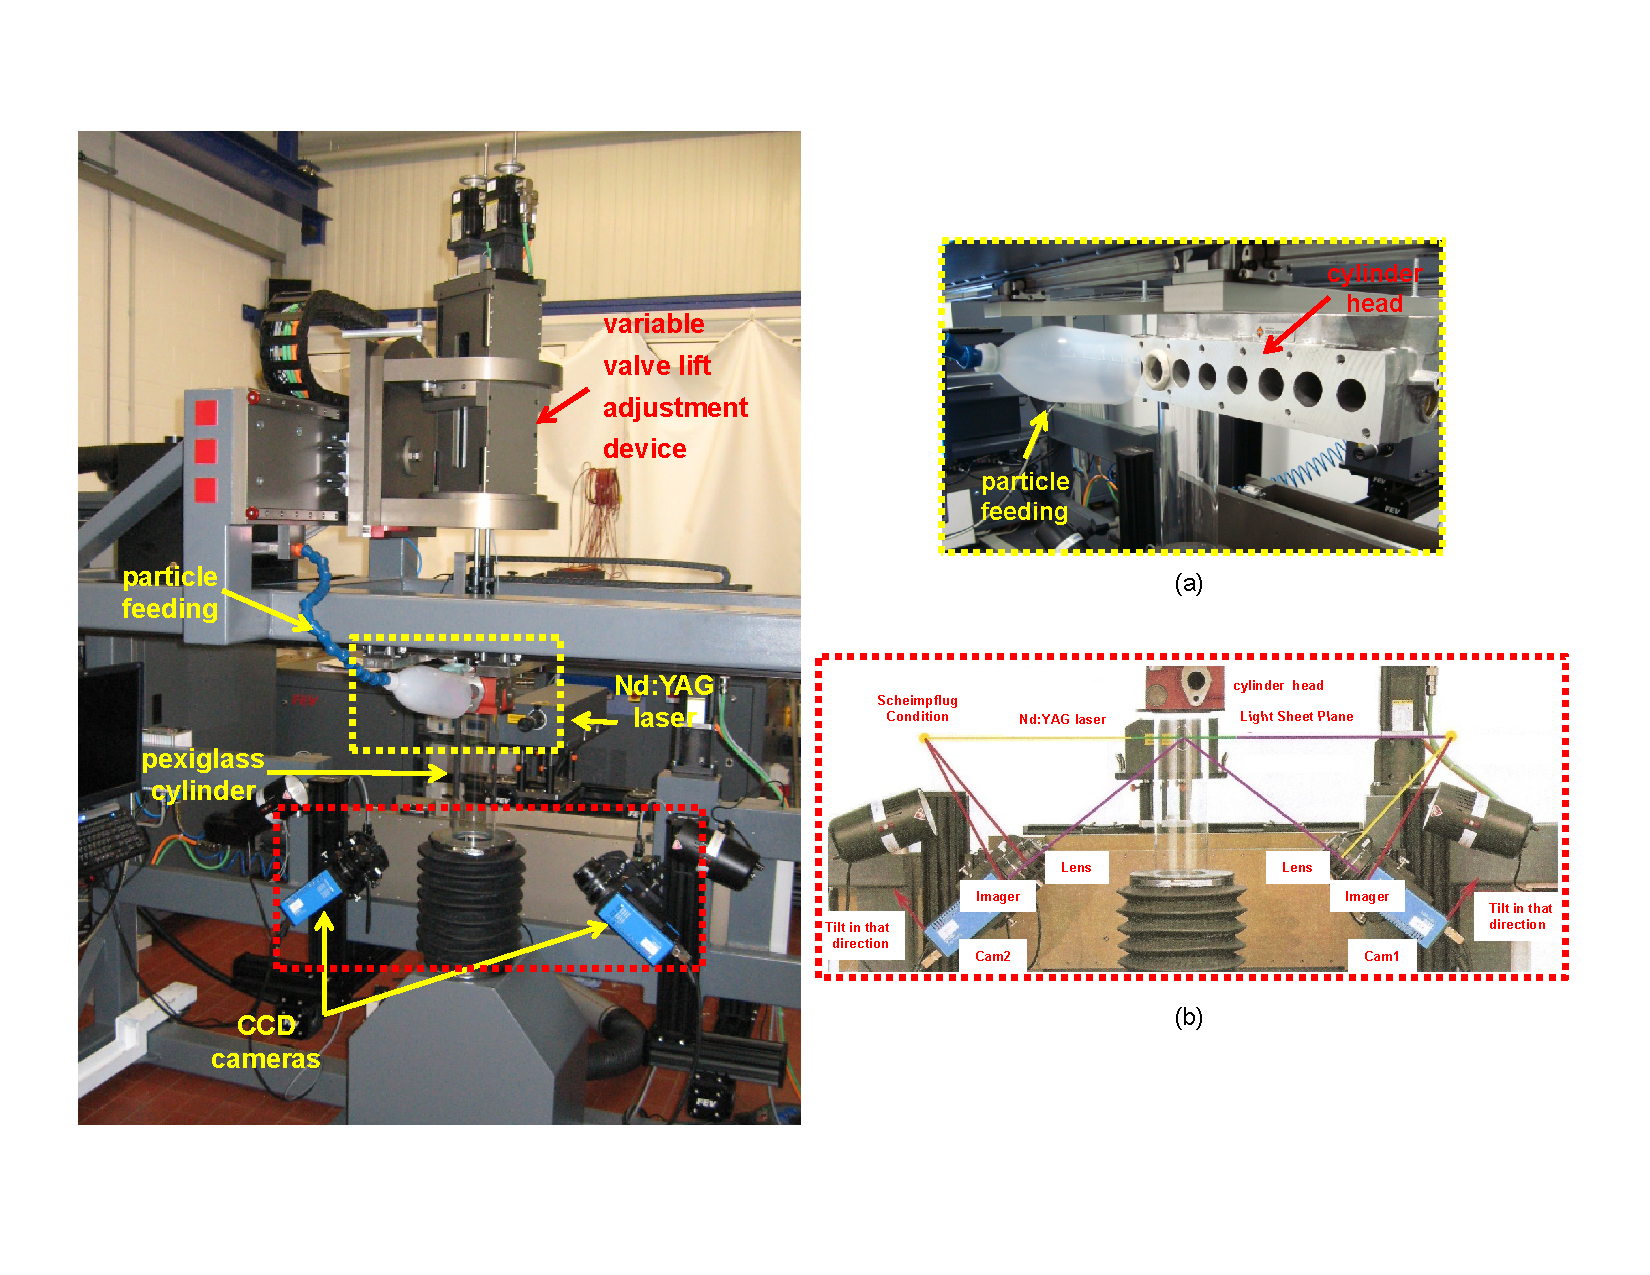
\includegraphics[width=1\textwidth]{./imgs/bench.pdf}
 \caption{Stereoscopic PIV test bench. (Left) Stereo PIV system; (Right) (a) Positioning of the particle feeding, (b) Scheimpflug configuration.}
 \label{fig: bench}
\end{figure}

The first step before starting the PIV experiment is the calibration that determines the metric on the measured plane, which is performed as follows. The horizontal laser sheet was aligned with a flat calibration target placed on top of the cylinder. After imaging the target a Tsai model (Tsai, 1987) was used to mapping pixel to real coordinates for each CCD camera. This model is based on pinhole camera model and describes radial lens distortions using nonlinear expression. Although the Tsai model employs more complex mapping function, it determines the position of CCD cameras for later reconstruction of the three-dimensional vector field. As the laser and the CCD cameras are installed on a three-axis traversing bench, different cross sections of the cylinder can be measured without requiring additional recalibration.

During the experiments, the pressure drop inside the cylinder has been kept constant at 4.9\,kPa by means of a blower bypass. The air flow is measured by a roots meter with simultaneous measurement of air temperature and pressure drop at the metering device.

The PIV measurements were taken on a cross section at distance D (cylinder diameter) bellows cylinder head face. A total of 100 frames pairs were recorded for each CCD camera at a frequency of 8\,Hz with a time interval between laser pulses of 10\,$\mu$s. The statistical sample size (100 frames) showed be enough for a precise flow decomposition. 

The tracer particle feeding was displaced close to the intake port of cylinder head and the particle flow has been adjusted until it was seen roughly 10 to 20 tracer particles in a typical 64x64\,pixel interrogation area, as shown in Fig.~\ref{fig: densityimage}. 

\begin{figure}[h]
 \centering
 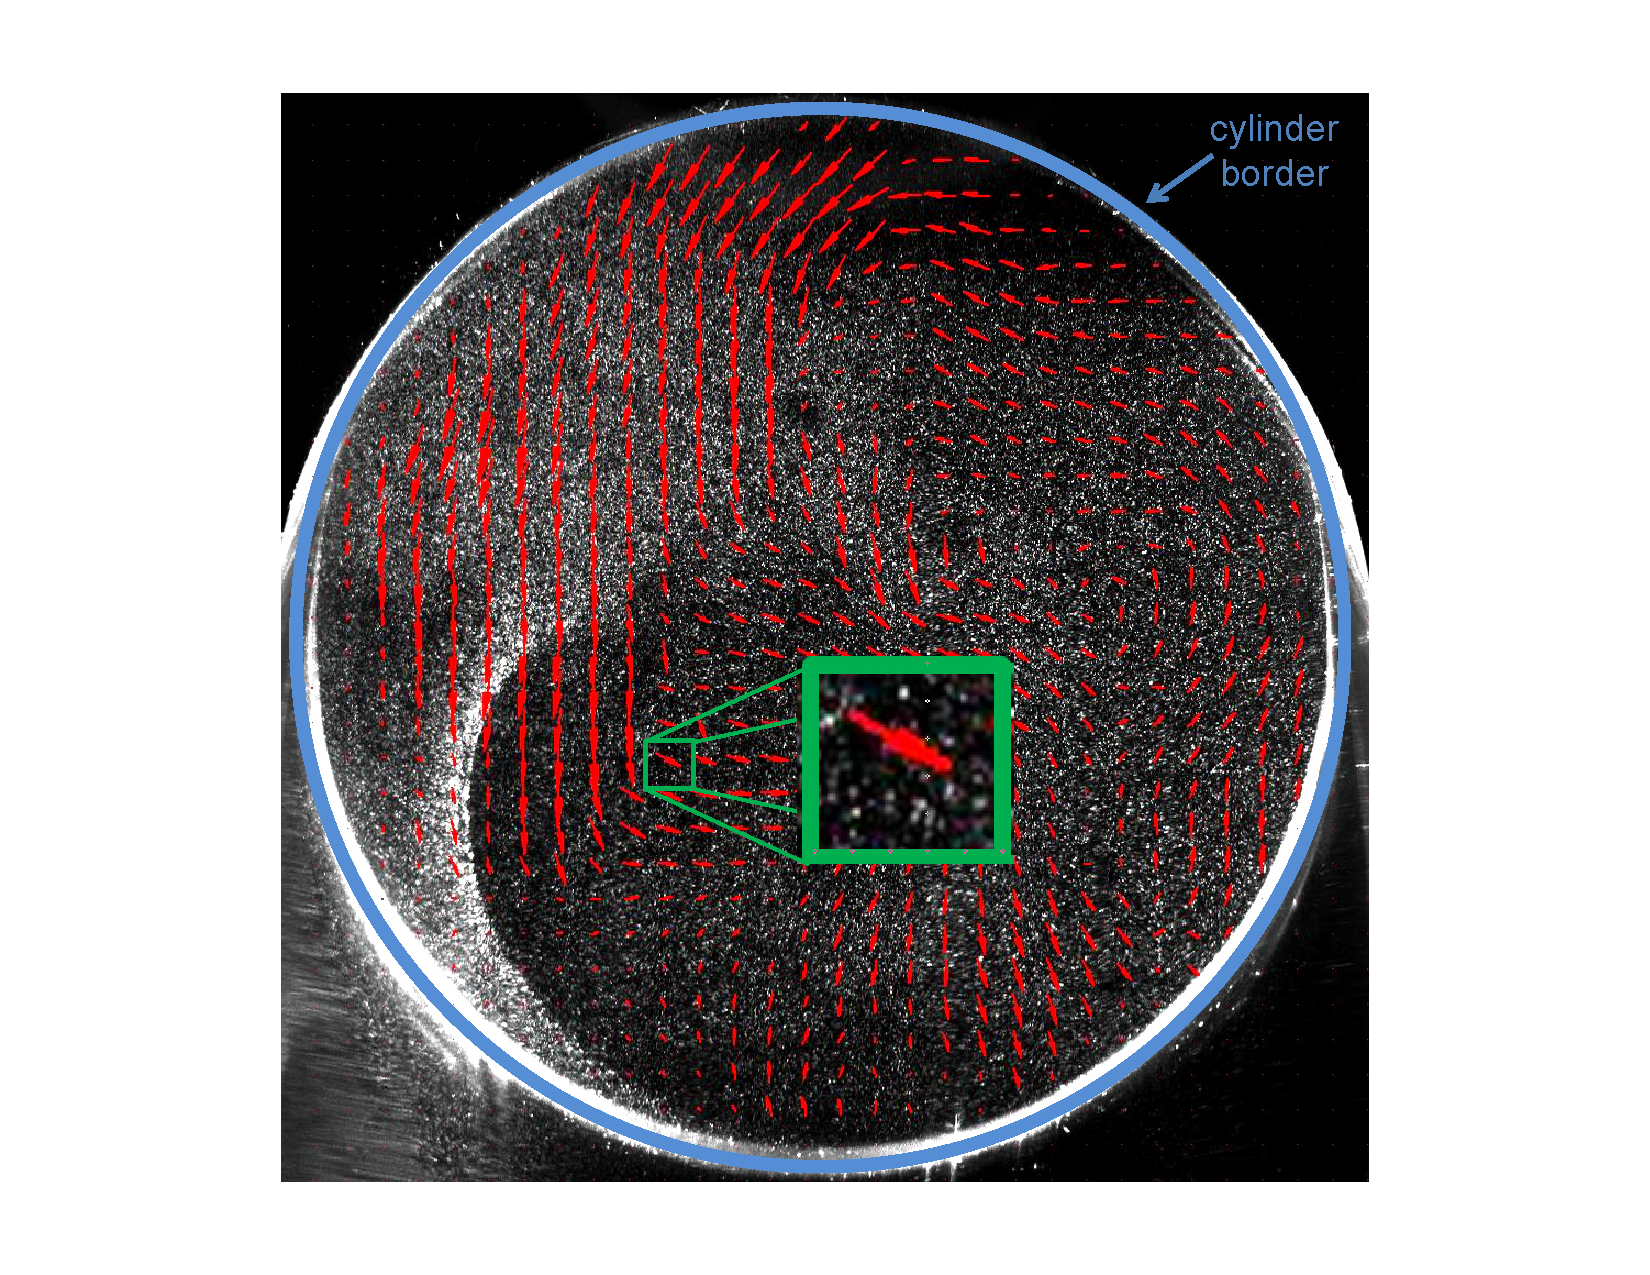
\includegraphics[width=0.4\textwidth]{./imgs/density.pdf}
 \caption{PIV sample image showing the calculated velocity field vectors over a cross section of an in-cylinder. Green square highlights a given interrogation area of 64x64 pixel. White dots are tracer particles.}
 \label{fig: densityimage}
\end{figure}

The PIV images were post-processed using multi-pass correlation to provide higher resolution vector data. A first correlation was started with a 64x64\,pixel interrogation size with 50$\%$ overlap followed by an adaptive cross-correlation with a final 32x32\,pixel interrogation size with 50$\%$ overlap. A median filter was applied in order to filter out outlier vectors. An interpolation algorithm based on a weighted mean technique was employed to replace the filtered velocity vectors. Finally, the perspective vector maps from each CCD camera were combined to obtain the third component velocity and to improve accuracy for the other two components.


\section{PROPER ORTHOGONAL DECOMPOSITION - SNAPSHOT METHOD}

The characterization of coherent structures is an interesting issue in the study of turbulent flows and it is the subject of vast literature (Heywood, 1988; Cosadia et al., 2006; Cazemier, 1997; Bergmann and Cordier, 2003, Hung and Hien, 1998; Boree, Maurel and Bazile, 2002; Li Y. et al., 2004). However, the mathematical definition of such structures is not necessarily standard and might differ depending on context. One possible way is the Proper Orthogonal Decomposition (POD) (Lumley, 1967), which establishes a criterium based on maximum energy content.

For optimizing the operation of an internal combustion engine, as previously mentioned in Section 1, the characterization of flow main structures is fairly important and the POD demonstrates to be an useful tool for their identification. As a favourable point, the efficiency of the decomposition increases with flow inhomogeneity such as those in the strong swirling flows sought in engine application. 

The main definitions used in the derivation of POD formulation are summarized below. Details of the theory might be found in Griffel (2002). Let's consider a set of $N$ observations (snapshots) of the flow velocity field denoted by $\left \lbrace \mathbf{U}_{s} : (1 \le s \le N) \in Z, \mathbf{U}_s \in \Omega \right \rbrace$, where $\Omega$ is the flow domain. $\bv{U}_{s}$ is the velocity field, a vector formed by the three velocity components $\bv{U}_{s}(\bv{x})=(u_1 (\bv{x}), u_2 (\bv{x}), u_3(\bv{x}))$. Due to the physical meaning of the velocity field, it is assumed that $\bv{U}_s \in L^2 (\Omega)$, where $L^2(\Omega)$ is the Hilbert space of the square-integrable functions (Riesz and Sz.-Nagy, 1990).

The observations can be the result of experimental measurements or computer simulations. These results may be not necessarily the flow velocity, but any of the flow properties. Furthermore, each observation must be taken in a different instant of time. In the present work, one observation is made up of the full procedure required by the PIV technique (as described in the Section 2) to provide a velocity field in some instant of time. The frames are taken at different times equally spaced and each event is assumed linearly independent.

The proper orthogonal decomposition consists in decomposing the set of observations in an orthonormal basis which ensures an extra condition for its elements (or modes, the nomenclature used hereafter). Thus, the velocity field can be represented by a series expansion in terms of the modes:


\begin{equation}\label{eq: Us}
 \bv{U}_s (\bv{x}) = \sum_{j=1}^{N} b^{s}_{j} \bv{\Phi}_{j}(\bv{x}) \,,
\end{equation}
\\
where $b^{s}_{j}$ is the time-dependent amplitude coefficient and the $\bv{\Phi}_{j}(\bv{x})$ is the set of vectors generating the POD basis.  
Each mode might be understood as a coherent structure.

These functions will be the most similar to the members of $\bv{U}_{s}$ on average if the normalized average projection of $\bv{U}_{s}$ onto $\bv{\Phi}$ is maximum:


\begin{equation}\label{eq: max-cond}
max \left \lbrace \frac{1}{N} \sum_{s=1}^{N} | \left(\bv{U}_{s} , \bv{\Phi}\right) |^2 \right \rbrace \quad \text{with} \quad (\bv{\Phi},\bv{\Phi}) =  \parallel \bv{\Phi} \parallel^2 = 1 \quad \text{and} \quad \bv{\Phi} \in L^2 (\Omega) \,,
\end{equation}
\\
where $(.,.)$ denotes the inner product associated with the norm $\parallel . \parallel$. The inner product of two vector fields $\bv{F}$ and $\bv{G}$ is defined as $(\bv{F},\bv{G}) \equiv \int_{\Omega} {\bv{F} \cdot \bv{G}} dS$, and the norm by $\parallel \bv{F} \parallel = \sqrt{(\bv{F},\bv{F})}$.


If it is made the assumption of linearly independent observations, the $\bv{\Phi}$ functions might be written as a linear combination of them:


\begin{equation}\label{eq: phifunctions}
 \bv{\Phi}_s = \sum_{j=1}^{N} a^{s}_{j} \bv{U}_{j}(\bv{x}) \,.
\end{equation}


The maximisation, Eq.~\eqref{eq: max-cond}, would be solved if all the coefficients $a^{s}_{j}$ in Eq.~\eqref{eq: phifunctions} were determined. For this purpose, let's define an integral operator $\bv{R}$ with kernel $\bv{K}$ given by:


\begin{equation}\label{KandR}
 \bv{K} (\bv{x}, \bv{x}^{\prime}) \equiv \frac{1}{N} \sum_{s=1}^{N} \bv{U}_s (\bv{x}) \bv{U}_s (\bv{\xp}) \quad \text{and} \quad \bv{R} \bv{\Phi} \equiv \int_{\Omega} \bv{K} (\bv{x}, \bv{x}^{\prime}) \cdot \bv{\Phi}(\bv{x}^{\prime}) dS^{\prime} \,,
\end{equation}
\\
where $\bv{K}=\sum_{s=1}^{N} (u_i u_j)_s$ is a tensor of second rank (a three-by-three matrix) and $\bv{R} \bv{\Phi}$ is a vector of three components. Both are composed of $L^2(\Omega)$ functions. As mentioned previously, from the physical nature of the velocity field, the elements of $\bv{K}$ satisfy:


\begin{equation}\label{eq: kernel}
 \int_{\Omega} | k_{ij} (\bv{x},\bv{\xp}) |^{2} dS < \infty \,.
\end{equation}


In this case, for a measure space $\Omega$, the linear integral operator on $L^{2}(\Omega)$ with kernel K is compact if $\int_{\Omega} | K( \bv{x})|^2 \bv{dx} \quad$ converges.  

Performing some algebraic manipulation, it is possible to show two properties of $\bv{R}$: non-negativeness and self-adjointness. The follow equation shows the non-negativeness of $\bv{R}$:


\begin{equation}\label{st1}
% (\bv{R}\bv{\Phi},\bv{\Phi}) = \sum_{i=1}^{N} | \left( \bv{\Phi} , \bv{U}_i\right) |^2 \ge 0\\
 \begin{split}
 (\bv{R}\bv{\Phi},\bv{\Phi}) &= \int_{\Omega} \bv{R}\bv{\Phi}(\bv{x}) \bv{\Phi}(\bv{x}) dS \\
 &= \int_{\Omega} \int_{\Omega} \bv{K}(\bv{x},\bv{\xp}) \bv{\Phi}(\bv{\xp}) dS^{\prime} \bv{\Phi}(\bv{x}) dS \\
 &= \frac{1}{N} \sum_{i=1}^{N} \int_{\Omega} \int_{\Omega} \bv{U}_{i}(\bv{x}) \bv{U}_{i}(\bv{\xp}) \bv{\Phi}(\bv{\xp}) dS^{\prime} \bv{\Phi}(\bv{x}) dS \\
 &= \frac{1}{N} \sum_{i=1}^{N} | \left(\bv{U}_{i} , \bv{\Phi}\right) |^2 \ge 0 \,.
 \end{split}
\end{equation}


Now, Equation~\eqref{st2} shows the self-adjointness of $\bv{R}$:


\begin{equation}\label{st2}
 \begin{split}
 (\bv{R}\bv{\Phi},\bv{\Psi}) &= \int_{\Omega} \left (\int_{\Omega} \bv{K}(\bv{x},\bv{\xp}) \cdot \bv{\Phi}(\bv{x}) dS \right) \cdot \bv{\Psi}(\bv{\xp}) dS^{\prime} = 
\int_{\Omega} \left( \int_{\Omega} \bv{K}(\bv{x},\bv{\xp}) \cdot \bv{\Psi}(\bv{\xp}) dS^{\prime} \right) \cdot \bv{\Phi}(\bv{x}) dS \\
 &= (\bv{\Phi},\bv{R}\bv{\Psi}) \quad \text{for all} \bv{\Phi}, \bv{\Psi} \in L^{2}(\Omega) \,.
\end{split}
\end{equation}

With these two properties of $\bv{R}$, the problem of maximizing Eq.~\eqref{eq: max-cond} is thus equivalent to a Rayleigh quotient e.g. if $\lambda$ is the largest eigenvalue of a positive self-adjoint compact operator, $\bv{A}$, on a Hilbert space $L^2 (\Omega)$, $\lambda = max \left\lbrace \bv{R(x)} : \bv{x} \in L^2 (\Omega) \right\rbrace$ where $\bv{R(x)=(x,Ax)/(x,x)}$, then:


\begin{equation}\label{eig1}
 \left(\bv{R} \bv{\Phi} , \bv{\Phi} \right) = \lambda \quad \text{with} \quad \parallel \bv{\Phi} \parallel = 1 \,.
\end{equation}


Thus, the Equation~\eqref{eig1} can be rewritten by the follow way:


\begin{equation}\label{eig2}
 \begin{split}
 \left(\bv{R} \bv{\Phi} , \bv{\Phi} \right) &= \lambda \parallel \bv{\Phi} \parallel \,; \\
 \left(\bv{R} \bv{\Phi} , \bv{\Phi} \right) &= \lambda \left(\bv{\Phi}, \bv{\Phi} \right) \, .
 \end{split}
\end{equation}


As $\lambda$ is a real positive eigenvalue: $\lambda \left(\bv{\Phi}, \bv{\Phi} \right) = \left(\lambda \bv{\Phi}, \bv{\Phi} \right)$. So:


\begin{equation}\label{eig3}
 \left(\bv{R} \bv{\Phi} , \bv{\Phi} \right) - \left(\lambda \bv{\Phi}, \bv{\Phi} \right) = 0 \,.
\end{equation}


Applying the additivity property of an inner product on the Eq.~\eqref{eig3} we have:


\begin{equation}\label{eig4}
 \left(\bv{R} \bv{\Phi} - \lambda \bv{\Phi}, \bv{\Phi} \right) = 0 \,.
\end{equation}


According to Eq.~\eqref{eq: max-cond}, $\bv{\Phi}$ can not be zero because his norm equals one. Therefore:

\begin{equation}\label{eig5}
 \bv{R} \bv{\Phi} = \lambda \bv{\Phi} \,.
\end{equation}


Replacing the Eq.~\eqref{eq: phifunctions} and Eq.~\eqref{KandR} on the Eq.~\eqref{eig5} we obtain:


\begin{equation} \label{eq: substituting} 
\int_{\Omega}  \left[\frac{1}{N} \sum_{i=1}^{N} \bv{U}_i(\bv{x})\bv{U}_i(\bv{x}) \right] \cdot \left[\sum_{j=1}^{N} a^{s}_{j} \bv{U}_{j}(\bv{\xp}) \right] dS^{\prime} = \lambda_{s} \sum_{i=1}^{N} a^{s}_{j} \bv{U}_{j} (\bv{x}) \,.
\end{equation}


Applying the dyadic product property $(\mathbf{u} \mathbf{v}) \cdot \mathbf{w} =  (\mathbf{v} \cdot \mathbf{w}) \mathbf{u}$ in Eq.~\eqref{eq: substituting}:


\begin{equation*}
\sum_{i=1}^{N} \left \lbrace \sum_{j=1}^{N} \left[\int_{\Omega} \frac{1}{N} \bv{U}_i(\bv{x}) \cdot \bv{U}_{j} (\bv{x}) dS^{\prime}  \right] a^{s}_{j} \right \rbrace \bv{U}_i(\bv{x}) = \lambda_{s} \sum_{j=1}^{N} a^{s}_{j} \bv{U}_{j} (\bv{x}) \,.
\end{equation*}


A sufficient condition for the equality to hold is:


\begin{equation}
\left[\frac{1}{N} \sum_{j=1}^{N} \int_{\Omega} \bv{U}_{i}(\bv{x}) \cdot \bv{U}_{j}(\bv{x}) dS^{\prime} \right] a^{s}_{j}= \lambda_{s} a^{s}_{j} \,.
\end{equation}


This expression can be written in matricial form according to the definitions below:


\begin{equation} \label{cov1}
\bv{C}_{N \times N} \bv{A}_{N \times 1} = \lambda \bv{A}_{N \times 1} \,,
\end{equation}


\begin{equation*}
\text{where} \, \, C_{ij}= \frac{1}{N}  \int_{\Omega} \begin{bmatrix}  \bv{U}_i(\bv{x}) \cdot \bv{U}_{j} (\bv{x})  \end{bmatrix}_{N \times N} dS^{\prime} \,.
\end{equation*}


Each eigenvector of Eq.~\eqref{cov1} will provide the $a^{s}_{j}$ coefficients of a POD basis element $\bv{\Phi}_s$, which can be obtained by computing Eq.~\eqref{eq: phifunctions}. Each eigenvalue $\lambda_s$ represents the time average kinetic energy of the correspondent mode. For notation purposes, the modes are ordered by the decreasing eigenvalue, so that the average energy content of $\bv{\Phi}_1$ is greater than $\bv{\Phi}_2$ and so on.

Due to the optimality condition imposed by the POD, Eq.~\eqref{eq: max-cond}, the convergence of the energy spectrum is faster than any other possible decomposition (in the sense of the average and the inner product defined in this paper).

The data provided by the PIV system consists of a regular 2D mesh with measured values positioned at grid nodes. Since the POD analysis will require surface integration, the nodes were grouped in triangular cells created by the Delaunay algorithm. The node values were then linearly interpolated to cell geometric centers and the surface integral of a property over a cell was computed from the following simple approximation,

\begin{equation}
 \int_{\Omega_i} \phi (\bv{x}) dS \approx \phi (\bv{x}_{CG}) S \,.
\end{equation}

After performing the integrations and having the matrix $C$ (Eq.~\eqref{cov1}), the computation of eigenvalues and eigenvectors is carried out with the opensource library SciPy.

\section{RESULTS}

The flow field of four different intake ports, namely \textit{Head 1, 2, 3} and \textit{4}, were measured in the stereoscopic PIV test bench for one valve lift fixed at 12\,mm.  Further, the flow field of Head 1 and 4 were also measured for a valve lift of 2\,mm.

The Figure~\ref{fig: energy_fraction} shows the content of time average energy in modes. The energy fraction content in each mode is presented by Fig.~\ref{fig: energy_fraction}(a). The Figure~\ref{fig: energy_fraction}(b) shows the cumulative energy when the modes are grouped from $\bv{\Phi}_1$ to $\bv{\Phi}_{100}$. For higher valve lifts, the flow field has shown more organized in the sense that more energy is stored in few modes. Only the first mode, $\bv{\Phi}_1$, contains up to 80$\%$ of the total energy (see the zoom of the Fig.~\ref{fig: energy_fraction}(a)). Moreover, from the 30$^{th}$ mode, the energy decreases following an exponential decay. The exponential law is given by $E(k) \approx a_1 e^{a_2 k} ,  k \ge 30$. The exponential constant ($a_2$) is in the interval of $[-0.031,-0.023]$ for all cases.


\begin{figure}[h]
\begin{tabular}{cc}
 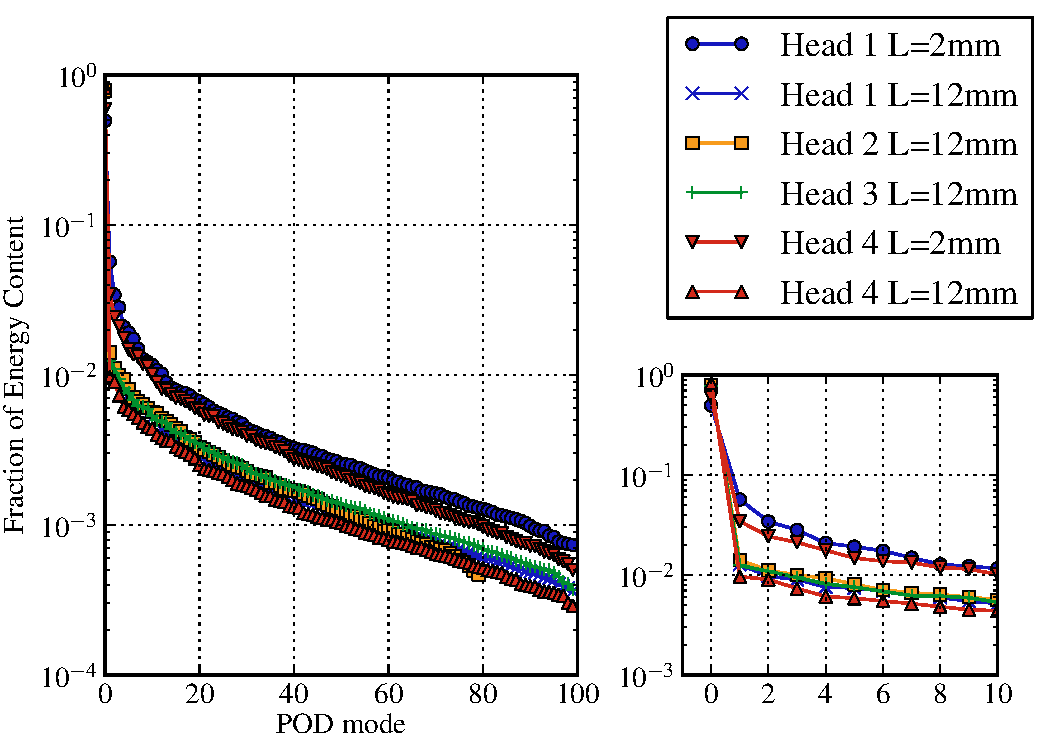
\includegraphics[width=0.5\textwidth]{./imgs/energy_spectra.pdf} & 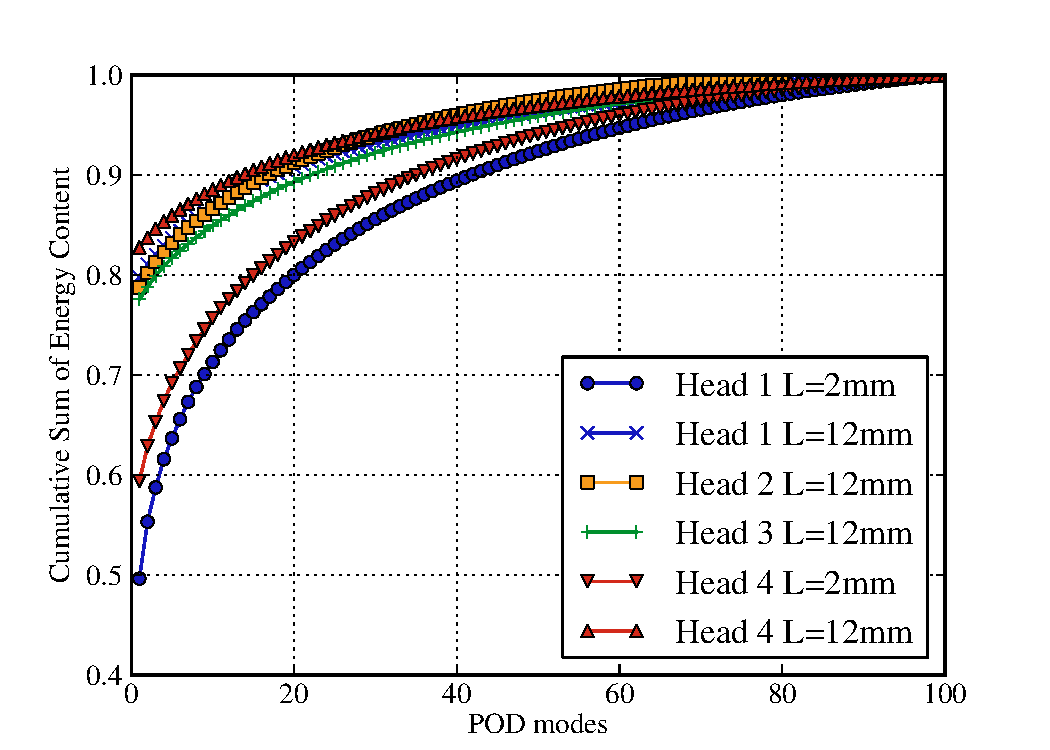
\includegraphics[width=0.5\textwidth]{./imgs/cumulative_energy.pdf} \\
(a) & (b)
\end{tabular}
 \caption{(a) Fraction of energy in each mode for all tested heads. The small frame is zooming the interval of $[0,10]$. (b) Cumulative energy, that is, the sum of the contributions from $\bv{\Phi}_1$ to some $\bv{\Phi}_k$.}
 \label{fig: energy_fraction}
\end{figure}


\begin{figure}[h]
 \centering
 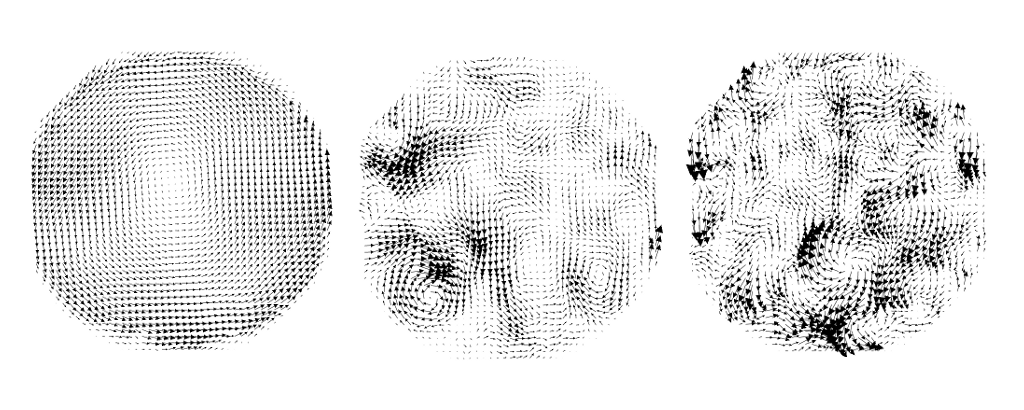
\includegraphics[width=0.78\textwidth]{./imgs/scania-modes.png}
 % scania-modes.png: 2196x879 pixel, 72dpi, 77.46x31.01 cm, bb=
 \caption{Velocity fields of Head 2: $\bv{\Phi}_1$ (left), $\bv{\Phi}_{15}$ (center) and $\bv{\Phi}_{30}$ (right).}
 \label{fig: organization}
\end{figure}

\clearpage

The link between energy content and the flow organization is supported by the observation of the mode velocity field presented in Fig.~\ref{fig: organization}. Here, the vector magnitudes are normalized according to the same norm defined in Eq.~\eqref{eq: max-cond}. It is possible to notice that the motion organization decreases with the higher order modes. Furthermore, these modes presents several vortical structures while the first mode contains the majority of swirling structure. Hence, $\bv{\Phi}_1$ have the majority of the angular momentum. 

So far, only the time averaged energy has been discussed. However, if the $b^{s}_{j}$ coefficients from Eq.~\eqref{eq: Us} are computed, the energy time history is recovered. The Figure~\ref{fig: energy_hist} presents the energy history for the first mode and the set of the first ten modes. It is seen that the first mode is in general more oscillatory when viewed separately in the gray line.  This is rather consistent since energy transfers between the modes are expected. The energy decrease in the first mode possibly increases the energy of some other mode in the set and the other way around. This energy transfer will reduce the oscillations.

The Figure~\ref{fig: Lz} shows the contribution of each mode to angular momentum around the cylinder axis. It is observed that the first mode contains the main swirling motion while the subsequent modes corresponds to the oscillating motion as shown in Fig.~\ref{fig: organization}. As one could expect, the low valve lift of 2\,mm did not clearly define swirl motion because of great magnitude oscillations.

In order to define which intake port geometry will better perform, in terms of increase the turbulence level close to spark ignition event, not only the energy in the modes most be analyzed but also their respective angular momentum. As showed in Fig.~\ref{fig: energy_hist}, the results (c) and (d) have a similar energy history level in the first mode and for the set of ten modes. It is mean that the Head 2 and 3 distribute the energy in a similar way. This same trend is also observed in terms of energy spectra (see Fig.~\ref{fig: energy_fraction}). However, the angular momentum is quite different as presented in Fig.~\ref{fig: Lz} by the plots (c) and (d). Comparing the results of the first mode velocity field presented by Fig.~\ref{fig: scaniavssygma}, it is noticed that the Head 3 velocity field is composed by two-vortex structure against only one big vortex in the Head 2. This is the main reason in the angular momentum production.


\begin{figure}[h]
 \centering
 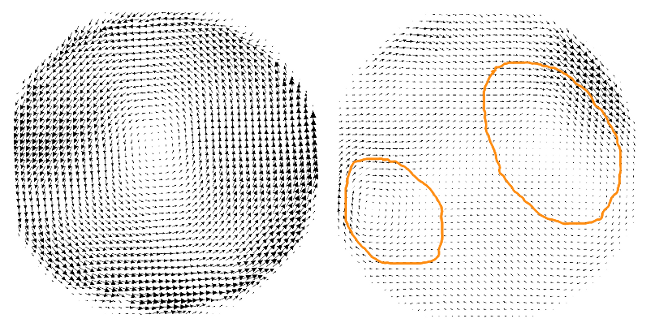
\includegraphics[width=0.6\textwidth]{./imgs/scania-vs-sygma.png}
 % scania-vs-sygma.png: 1429x740 pixel, 72dpi, 50.41x26.10 cm, bb=
 \caption{Velocity field of the first mode ($\bv{\Phi}_1$) for the Heads 2 (left) and 3 (right). The orange lines highlight the two vortex structure formed by the Head 3 in contrast to the one big vortex of Head 2.}
 \label{fig: scaniavssygma}
\end{figure}


\begin{figure}[h]
\begin{tabular}{cc}
 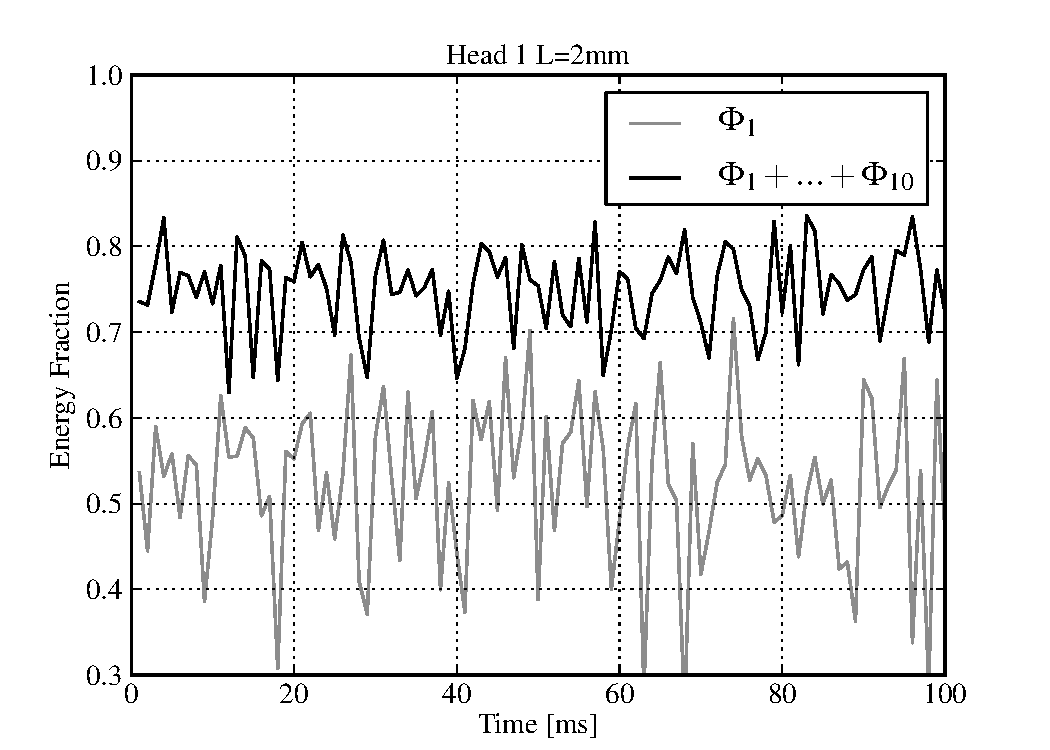
\includegraphics[width=0.5\textwidth]{./imgs/energy1.pdf} & 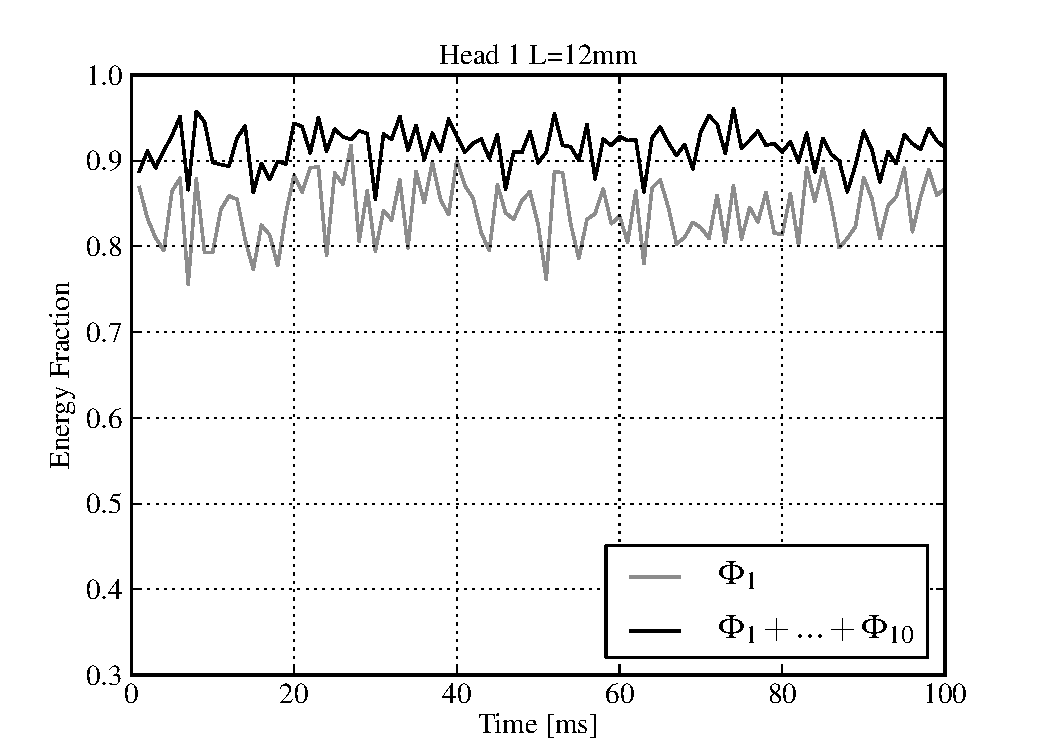
\includegraphics[width=0.5\textwidth]{./imgs/energy2.pdf} \\
(a) & (b) \\
 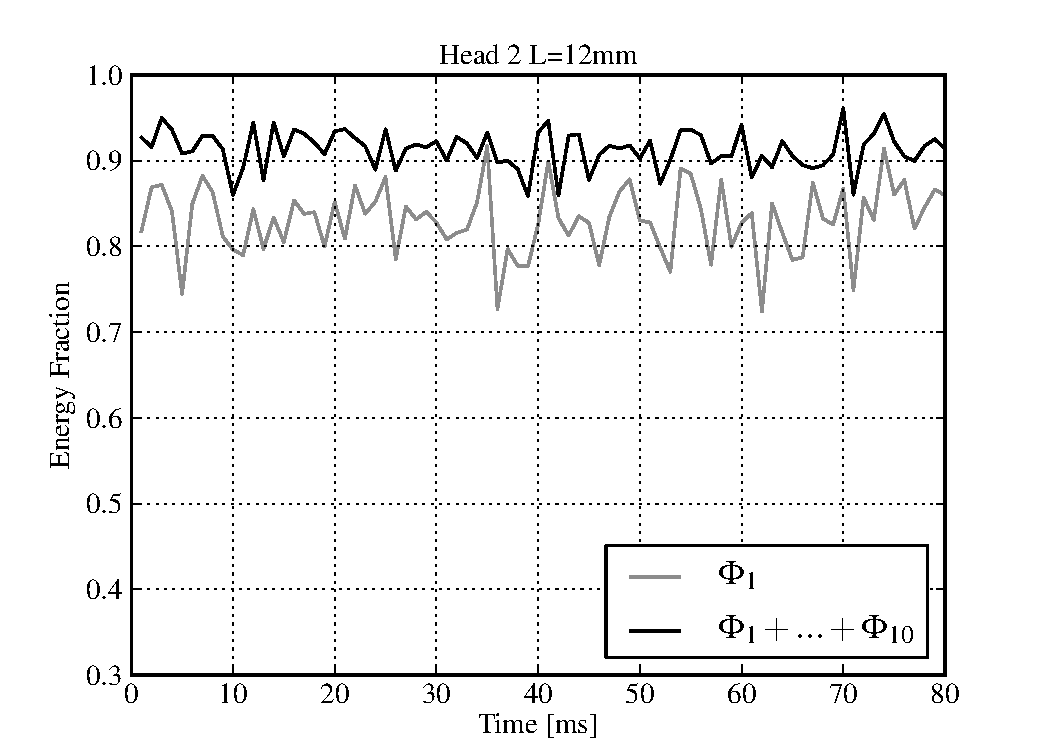
\includegraphics[width=0.5\textwidth]{./imgs/energy3.pdf} & 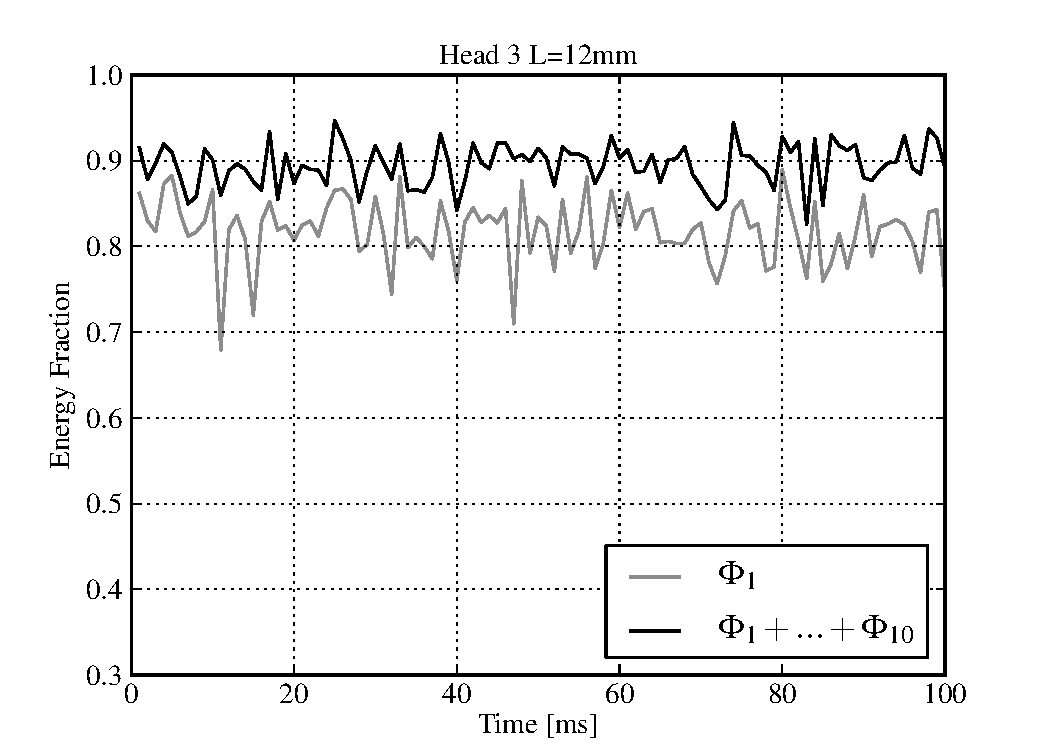
\includegraphics[width=0.5\textwidth]{./imgs/energy4.pdf} \\
(c) & (d) \\
 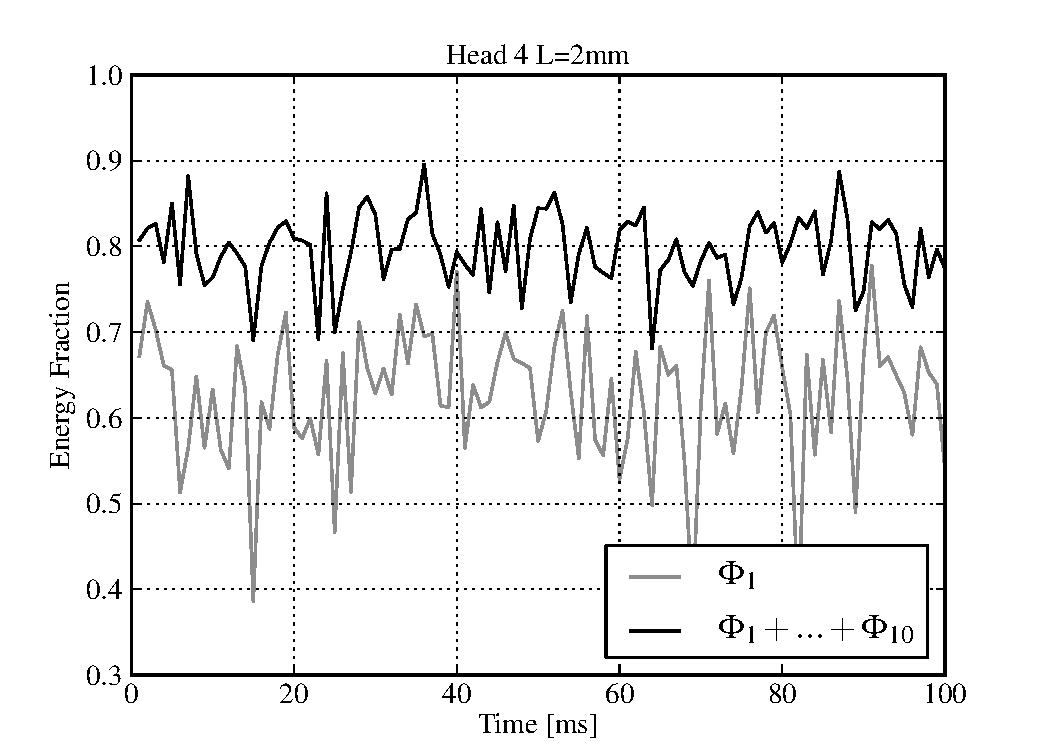
\includegraphics[width=0.5\textwidth]{./imgs/energy5.pdf} & 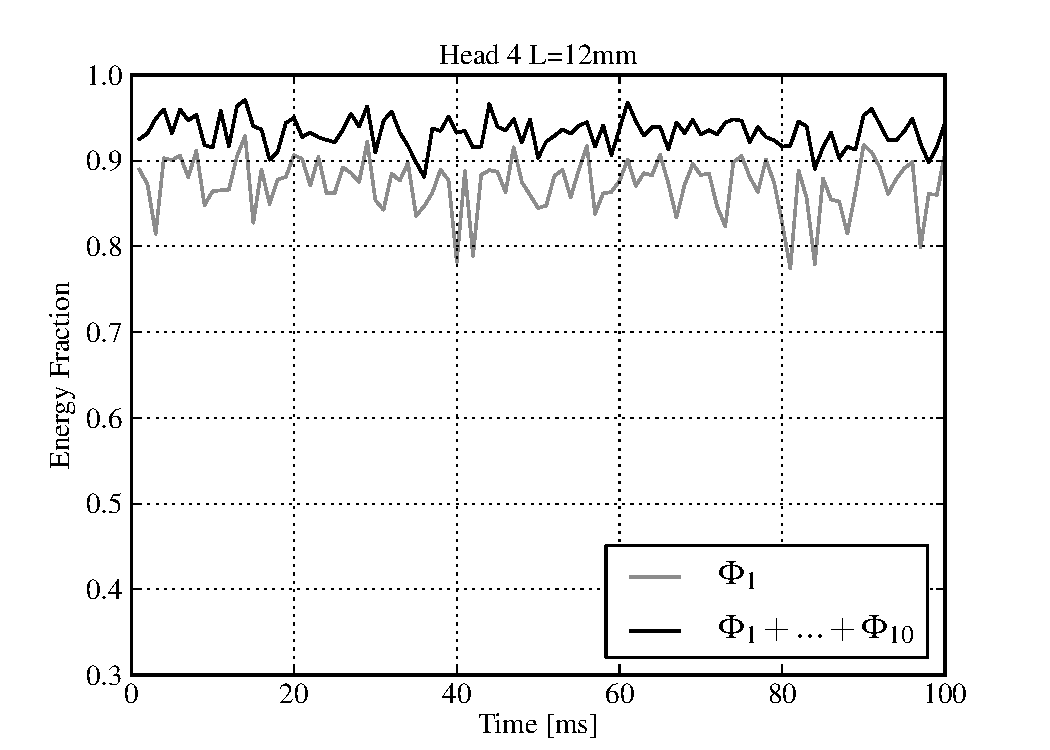
\includegraphics[width=0.5\textwidth]{./imgs/energy6.pdf} \\
(e) & (f)
\end{tabular}
 \caption{Energy history for $\bv{\Phi}_1$ (gray line) and for $\bv{\Phi}_{1}+...+\bv{\Phi}_{10}$ (black line).}
 \label{fig: energy_hist}
\end{figure}


\begin{figure}[h]
\begin{tabular}{cc}
 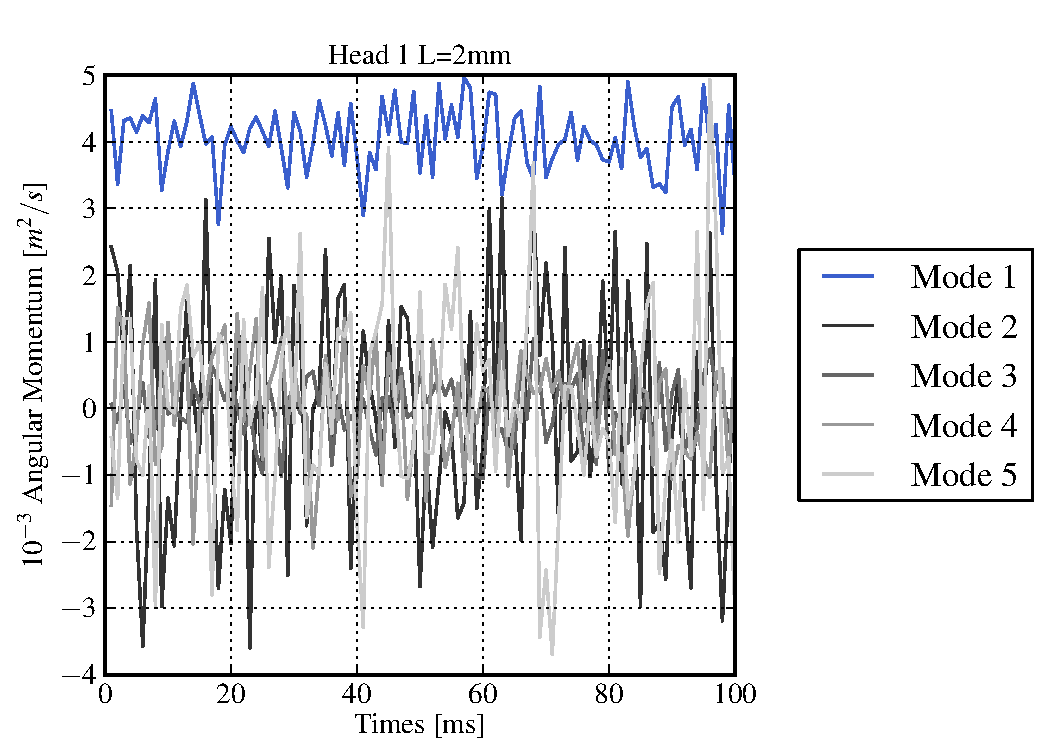
\includegraphics[width=0.5\textwidth]{./imgs/Lz_H1L2.pdf} & 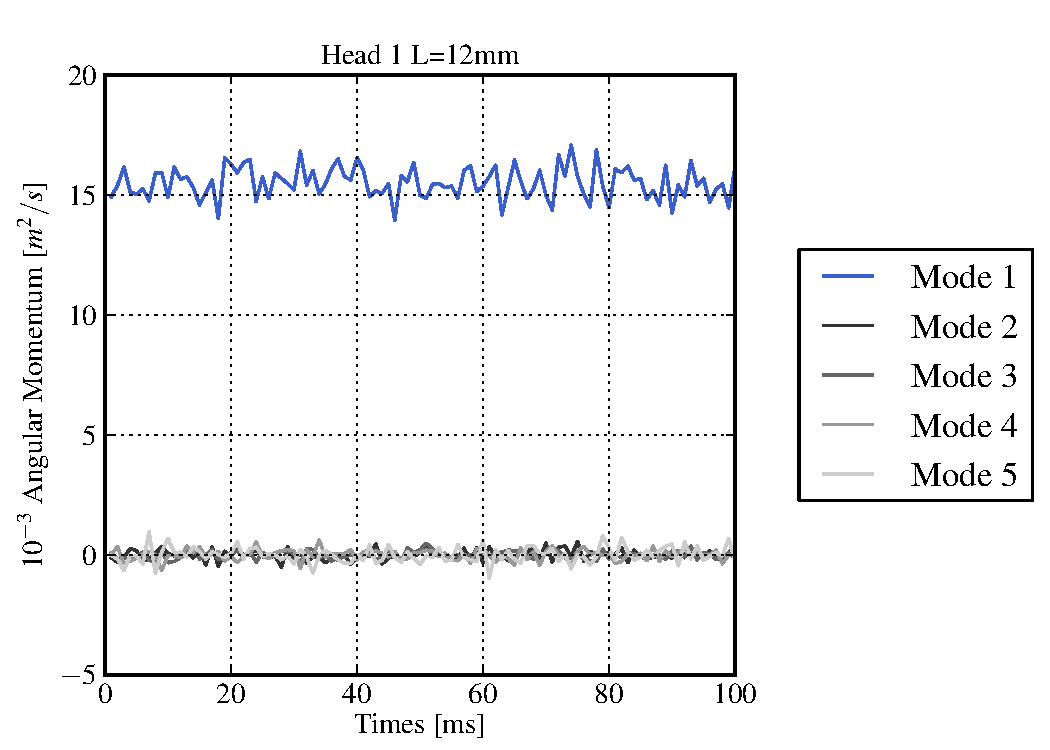
\includegraphics[width=0.5\textwidth]{./imgs/Lz_H1L12.pdf} \\
 (a) & (b) \\
 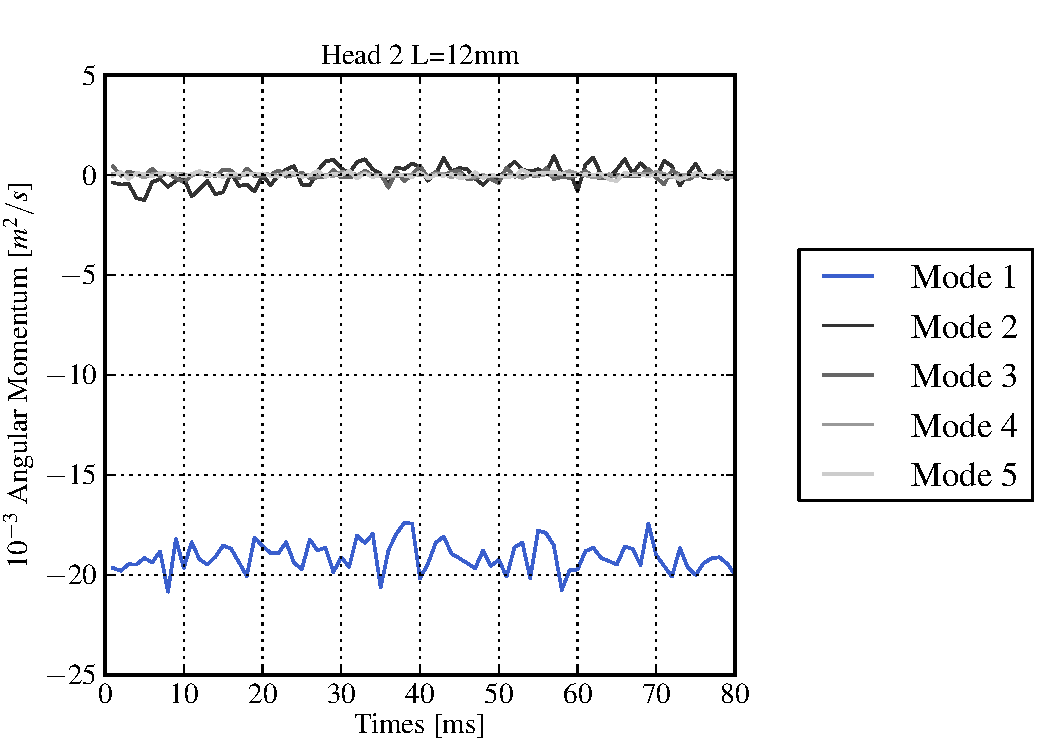
\includegraphics[width=0.5\textwidth]{./imgs/Lz_H2L12.pdf} & 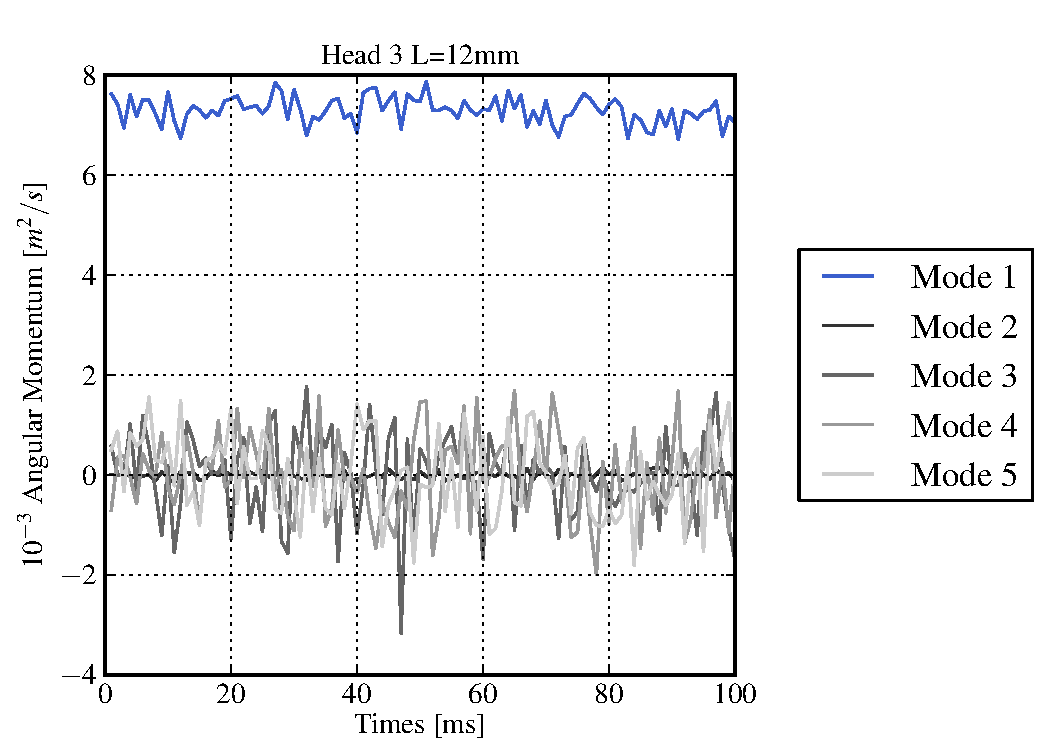
\includegraphics[width=0.5\textwidth]{./imgs/Lz_H3L12.pdf} \\
(c) & (d) \\
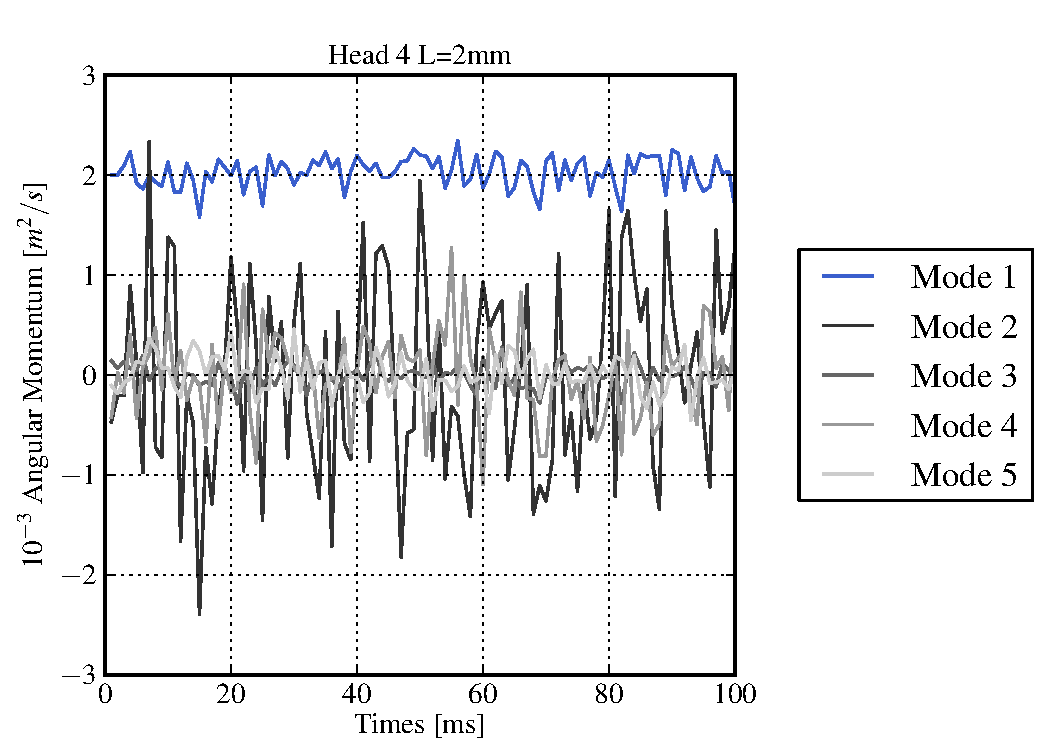
\includegraphics[width=0.5\textwidth]{./imgs/Lz_H4L2.pdf} & 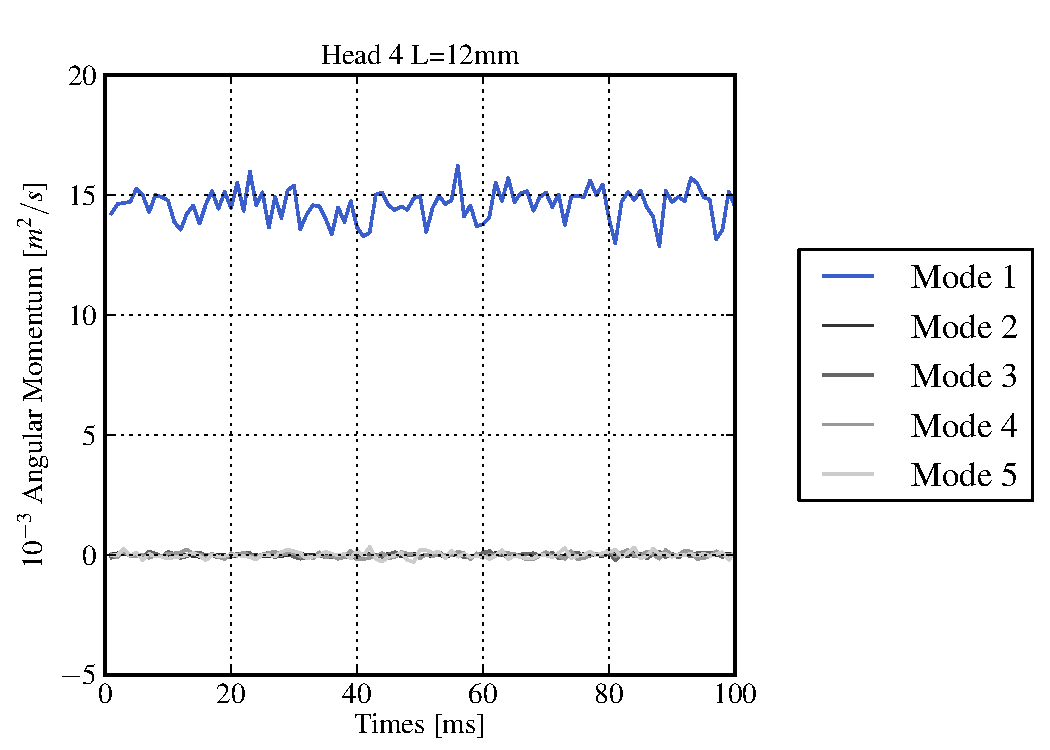
\includegraphics[width=0.5\textwidth]{./imgs/Lz_H4L12.pdf} \\
(e) & (f)
\end{tabular}
 \caption{Contributions to angular momentum of the first five modes.}
 \label{fig: Lz}
\end{figure}

\clearpage


\section{CONCLUSION}

In order to better understand how the intake ports geometry influence the flow which enters inside the combustion chamber during the intake phase, a statistical decomposition, like proper orthogonal decomposition, was applied on the three dimensional velocity flow field obtained with a stereoscopic PIV.

The results have shown that the first mode contains up to 80$\%$ of the time average kinetic energy of the flow field and have the major swirling structure. Therefore, the first mode defines the average angular momentum. The other modes, which we can call low energy modes, have shown several vortical structures, as presented in Fig.~\ref{fig: organization}, and have an average angular momentum around zero (see Fig.~\ref{fig: Lz}).

In what concerns the flow regularity, Fig.~\ref{fig: Lz} shows that the first mode basically defines the average angular momentum, which is superposed by the contributions of higher modes with average angular momentum around zero. Looking for the differences from one port to another, $\bv{\Phi}_1$ is much more disturbed by higher modes in the case of Head 3. This implies in having more dispersed swirling structures in the engine when concerning the ensemble of different cycles. It is also notable the regularity of Head 4, for which all oscillations are rather small.

Even if a mean swirl is measured, we have shown that the structure of the mean flow is complex and difficult to interpret. Thus, POD has shown itself to be an important methodology to analyze the flow and an important tool for the design of the cylinder head.


\section{ACKNOWLEDGEMENTS}

The authors gratefully thanks the Vale Solu\c{c}\~{o}es em Energia (VSE) for the laboratory structure installed in S\~{a}o Jos\'{e} dos Campos-SP.


\section{REFERENCES}

\begin{thebibliography}{1}
\bibitem[Bergmann and Cordier, 2003]{bergmann} Bergmann M. and Cordier L., 2003, "Post-Processing of Experimental and Numerical Data", Lecture of Von Karman Institute for Fluid Dynamics.
\bibitem[Boree, Maurel and Bazile, 2002]{tumble} Boree J., Maurel S. and Bazile R., 2002, "Disruption of a compressed vortex", Physics of Fluids.
\bibitem[Cazemier, 1997]{podthesis} Cazemier, W., 1997, "Proper Orthogonal Decomposition and Low Dimensional Models for Turbulent Flows", Ph.D Dissertation.
\bibitem[Cosadia et al., 2006]{cyclic}  Cosadia I., Bor\'{e} J., Charnay G. and Dumont P., 2006, "Cyclic variations of the swirling flow in a Diesel transparent engine", Experiments in Fluids.
\bibitem[Griffel (2002)]{griffel} Griffel, D. H., 2002, "Applied Functional Analysis", Dover Books on Mathematics.
\bibitem[Haworth et al., 2000]{Haworth} Haworth D.C., Cuenot B., Poinsot T.J. and Blint R.J., 2000, "Numerical Simulation of turbulent propane-air combustion with non-homogeneous reactants", Combustion $\&$ Flame 121, pp. 395-417.
\bibitem[H\'{e}lie and Trouv\'{e}, 2000]{Helie} H\'{e}lie J. and Trouv\'{e} A., 2000, "A modified coherent flame model to describe turbulent flame propagation in mixtures with variable composition", Proceedings of the Combustion Institute 28, pp.193-201.
\bibitem[Heywood, 1988]{heywood} Heywood, J. B. , 1988, "Internal Combustion Engine Fundamentals", McGraw-Hill International Editions.
\bibitem[Hung and Hien, 1998]{hung} Hung V. Ly and Hien T. Tran, 1998, "Proper Orthogonal Decomposition for Flow Calculations and Optimal Control in a Horizontal CVD Reactor", North Carolina State University.
\bibitem[Jim\'{e}nez et al., 2002]{Jimenez} Jim\'{e}nez C., Haworth D., Cuenot B. and Poinsot T.J., 2002, "Direct numerical simulation and modeling for lean stratified propane-air flames", Combustion $\&$ Flame 128, pp. 1-21.
\bibitem[Li Y. et al., 2004]{cyclic2} Li Y., Zhao H., Leach B., Ma T. and Ladommatos N., 2004, "Characterization of an in-cylinder flow structure in a high-tumble spark ignition engine", International Journal  of Engine Research.
\bibitem[Lumley, 1967]{Lumley} Lumley J. L., 1967, "The structure of inhomogeneous turbulence", In Yaglom, A.M., and Tatarski, V. I. (eds.), Atmospheric turbulence and wave propagation, Moscow,Nauka, pp.166-178.
\bibitem[Pasquier et al., 2007]{Pasquier} Pasquier N., Lecordier B., Trinit\'{e} M. and Cessou A., 2007, "An experimental investigation of flame propagation through a turbulent stratified mixture", Proceedings of the Combustion Institute 31, pp.1567-1574.
\bibitem[Poinsot and Veynante,2005]{poinsot} Poinsot, T. and Veynante, D., 2005, "Theoretical and Numerical Combustion",  R.T. Edwards.
\bibitem[Raffel et al., 2007]{Raffel} Raffel M., Willert C., Wereley S. and Kompenhans J., 2007, "Particle Image Velocimetry: A Practical Guide", Springer-Verlag Berlin Heidelberg.
\bibitem[Riesz and Sz.-Nagy,1990]{Riesz} Riesz F. and Sz.-Nagy B.,1990, "Functional analysis", New York:Dover.
\bibitem[Tsai, 1987]{Tsai} Tsai R.Y., 1987, "A versatile camera calibration technique for high-accuracy 3D machine vision metrology using off-the-shelf TV cameras and lenses", IEEE J. Robot. Autom.
\bibitem[Xiong and Roberts, 2002]{Xiong} Xiong Y. and Roberts W.L., 2002, "Observations on the interaction between a premixed flame kernel and a vortex of different equivalent ratio", Proceedings of the Combustion Institute 29, pp.1687-1693.

\end{thebibliography}

\end{document}
